% \documentclass{book}

% \usepackage{tikz}
% \usetikzlibrary{shapes.geometric}
% \usetikzlibrary{math}

% \usepackage{ifthen}
% \usepackage{listofitems}
% \usepackage{catchfile}

% %-----------------------------------------------------------
% % Drawing Stones

% % From [this answer by @DavidCarlisle](https://tex.stackexchange.com/a/708876/64441).
% \newcommand\notwhite{black}
% \newcommand\notblack{white}

% % From [this answer by @DavidCarlisle](https://tex.stackexchange.com/a/708893/64441).
% \ExplSyntaxOn
%   \cs_generate_variant:Nn \int_from_alph:n {e}

%   \NewExpandableDocumentCommand{\stringToCoordX}{ m }{
%     \int_from_alph:e { \use_i:nn #1 }
%   }
%   \NewExpandableDocumentCommand{\stringToCoordY}{ m }{
%     \boardSize + 1 - ~\int_from_alph:e { \use_ii:nn #1 }
%   }
% \ExplSyntaxOff

% \newcommand{\setCoords}[1]{
%   \pgfmathsetmacro{\x}{\stringToCoordX{#1} - 1}
%   \pgfmathsetmacro{\y}{\stringToCoordY{#1} - 1}
% }

% \newcounter{moveCounter}
% \setcounter{moveCounter}{1}

% \newcommand{\stepMoveCounter}{
%   \stepcounter{moveCounter}
% }

% %-----------------------------------------------------------
% % Drawing Stones and Moves

% \newcommand{\drawStoneFromSgfCoords}[2]{%
%   \setCoords{#2}

%   \draw[draw = \UseName{not#1}, fill = #1, line width = 0.1mm]
%     (\x * \step, \y * \step)
%     circle [radius = 0.2575cm];
% }

% \newcommand{\drawMoveFromSgfCoords}[2]{
%   \expandafter\xdef\csname thecolorat#2\endcsname{#1}% SAVE COLOR AT #2
%   \drawStoneFromSgfCoords{#1}{#2}
%   \textLabel{#1}{#2}{\themoveCounter}

%   \stepMoveCounter
% }

% %-----------------------------------------------------------
% % Labels

% \newcommand\StoneColor[1]{% COMPLEMENTARY COLOR OF REFERENCED STONE
%   \ifcsname thecolorat#1\endcsname
%     \csname thecolorat#1\endcsname
%   \else
%     white% COMPLEMENT OF DEFAULT LABEL COLOR WHEN NOT ATOP EXISTING STONE
%   \fi
% }

% \newcommand{\textLabel}[3]{%
%   \setCoords{#2}%

%   \draw (\x * \step, \y * \step) 
%   node[
%     color     = -\StoneColor{#2},
%     inner sep = 1pt
%   ] {#3};
% }

% \newcommand{\triangleLabel}[2]{
%   \setCoords{#2}

%   \draw (\x * \step, \y * \step) 
%     node[
%       isosceles triangle,
%       draw                          = #1,
%       color                         = -\StoneColor{#2},
%       fill                          = \StoneColor{#2},
%       minimum height                = \step * 10,
%       minimum width                 = \step * 10,
%       line width                    = 0.5mm,
%       rotate                        = 90,
%       isosceles triangle apex angle = 60,
%       inner sep                     = 0pt,
%     ] {};
% }

% %-----------------------------------------------------------
% % SGF Parser

% % From [this answer by @StevenB.Segletes](https://tex.stackexchange.com/a/709014/64441).
% \long\def\Firstof#1#2\endFirstof{#1}

% \newcommand\thecolorofB{black}
% \newcommand\thecolorofAB{black}
% \newcommand\thecolorofW{white}
% \newcommand\thecolorofAW{white}
% \newcommand\thecolorofMA{white}
% \newcommand\thecolorofCR{white}
% \newcommand\thecolorofTR{white}
% \newcommand\thecolorofSQ{white}
% \newcommand\thecolorofLB{white}

% \long\def\Keytypeof#1{\csname thekeytypeof#1\endcsname}

% \newcommand\thekeytypeofB{M}  % black move
% \newcommand\thekeytypeofAB{A} % added (edited) black stone
% \newcommand\thekeytypeofW{M}  % white move
% \newcommand\thekeytypeofAW{A} % added (edited) white stone
% \newcommand\thekeytypeofMA{K} % cross (mark) label
% \newcommand\thekeytypeofCR{C} % circle label
% \newcommand\thekeytypeofTR{T} % triangle label
% \newcommand\thekeytypeofSQ{S} % square label
% \newcommand\thekeytypeofLB{L} % text label

% \newcommand{\parseSgf}[1]{%
%   \setsepchar{(||)/;/]/[/:}%
%   \readlist*\Z{#1}%

%   \foreachitem \Branch \in \Z[]{%
%   \foreachitem \Group \in \Z[\Branchcnt]{%
%     \foreachitem \Key \in \Z[\Branchcnt, \Groupcnt]{%
%      \if\relax\Key\relax% IF BLANK KEY & VALUE, SKIP
%      \else
%       \itemtomacro\Z[\Branchcnt, \Groupcnt, \Keycnt, 1]\KeyName
%       \if\relax\KeyName\relax% IF VALUE, BUT NO KEYNAME, USE RECENT KEYNAME
%         \let\KeyName\MostRecentKeyname
%       \else
%         \xdef\MostRecentKeyname{\KeyName}%
%       \fi
%       \itemtomacro\Z[\Branchcnt, \Groupcnt, \Keycnt, 2, 1]\KeyValue

%       \edef\tmp{{\csname thecolorof\KeyName\endcsname}{\KeyValue}}%

%       \if\Keytypeof\KeyName M
%         \expandafter\drawMoveFromSgfCoords\tmp
%       \fi
%       \if\Keytypeof\KeyName A
%         \expandafter\drawStoneFromSgfCoords\tmp
%       \fi
%       \if\Keytypeof\KeyName K
%         \expandafter\crossLabel\tmp
%       \fi
%       \if\Keytypeof\KeyName C
%         \expandafter\circleLabel\tmp
%       \fi
%       \if\Keytypeof\KeyName T
%         \expandafter\triangleLabel\tmp
%       \fi
%       \if\Keytypeof\KeyName S
%         \expandafter\squareLabel\tmp
%       \fi
%       \if\Keytypeof\KeyName L
%         \expandafter\textLabel\tmp{\Z[\Branchcnt, \Groupcnt, \Keycnt, 2, 2]} 
%       \fi
%      \fi
%     }
%   }%
%   }%
% }

% % From [this question/answer](https://tex.stackexchange.com/a/726141/64441)
% \newcommand\parseSgfFile[1]{%
%   \CatchFileDef{\mysgf}{#1}{}%
%   \parseSgf{\mysgf}% 
% }

% %-----------------------------------------------------------
% % Grid

% \newcommand{\calculateStep}{
%   \pgfmathsetmacro{\step}{\boardDimension / (\boardSize - 1)} % chktex 1
% }

% % From [this answer by @UlrichDiez](https://tex.stackexchange.com/a/709341/64441).
% \pgfkeys{%
%   %---------------------------------------------------------
%   /phili/goGrid/.cd, 
%     %-------------------------------------------------------
%     % Dimensions
%     board dimension/.store in    = \boardDimension,
%     board dimension              = 10cm,
%     board size/.store in         = \boardSize,
%     board size                   = 19,
%     %-------------------------------------------------------
%     % Outline
%     outline line width/.store in = \boardOutlineWidth,
%     outline line width           = 0.7mm,
%   %---------------------------------------------------------
%   /phili/goban/.search also={/phili/goGrid},
%   /phili/goban/.cd,  
%     %-------------------------------------------------------
%     % Scale
%     scale/.store in              = \scale,
%     scale                        = 1,
%     %-------------------------------------------------------
%     % Partial Boards
%     horizontal clip start/.store in = \horClipStart,
%     horizontal clip start           = -1,
%     horizontal clip end/.store in   = \horClipEnd, % This is more like the width?
%     horizontal clip end             = -1,
%     vertical clip start/.store in   = \verClipStart,
%     vertical clip start             = -1,
%     vertical clip end/.store in     = \verClipEnd, % This is more like the height?
%     vertical clip end               = -1,
%   %---------------------------------------------------------
% }

% % Parameters
% %
% % - `board dimension` (in cm)
% % - `board size` (square)
% % 
% % Example: A 19x19 board with size 10cm x 10cm:
% %
% % ```tex
% % \goGrid[board dimension    = 10,
% %         board size         = 9,
% %         scale              = 1,
% %         outline line width = 0.5mm]
% % ```
% \newcommand{\goGrid}[1][]{
%   \pgfkeys{/phili/goGrid/.cd, #1}

%   \calculateStep

%   \draw[step=\step] (0, 0) grid
%     (\boardDimension, \boardDimension);
  
%   \boardOutline{\boardDimension}

%   \drawHoshis
% }

% % Reference: [Drawing a Non-Jagged Grid Outline](https://tex.stackexchange.com/q/709298/64441)
% %
% % Parameters
% %
% % 1: dimension (in cm)
% % 
% % Example: `\boardOutline{10}`
% \newcommand{\boardOutline}[1]{
%   \draw[step       = #1,
%         line width = \boardOutlineWidth,
%         line cap   = rect] 
%     (0, 0) grid (#1, #1);
% }

% % Example: A 19x19 board with size 10cm x 10cm: `\drawHoshis`
% \newcommand{\drawHoshis}{
%   \tikzmath{
%     \hoshiRadius = \step * 0.125;
%     %
%     \centerHoshi = ceil(\boardSize / 2);
%     %
%     int \hoshiDistance;
%     if \boardSize<12 then {
%       \hoshiDistance = 3;
%     } else {
%       \hoshiDistance = 4;
%     };
%     %
%     \hoshiComplement = \boardSize - \hoshiDistance + 1;
%   }

%   \drawCenterHoshi
%   \drawCornerHoshis
%   \ifnum\boardSize>6\relax
%     \drawCornerHoshis
%   \fi
%   \ifthenelse{\isodd{\boardSize}}{
%     \ifnum\boardSize>13\relax
%       \drawSideHoshis
%     \fi
%   }{}
% }

% \newcommand{\drawCenterHoshi}{
%   \pgfmathsetmacro{\centerHoshiCoord}{(\centerHoshi - 1) * \step}

%   \filldraw (\centerHoshiCoord, \centerHoshiCoord)
%     circle [radius=\hoshiRadius];
% }

% \newcommand{\drawCornerHoshis}{
%   \def\cornerHoshisArray{%
%     {\hoshiDistance, \hoshiDistance},%
%     {\hoshiComplement, \hoshiDistance},%
%     {\hoshiDistance, \hoshiComplement },%
%     {\hoshiComplement, \hoshiComplement}%
%   }

%   \loopOverHoshis{\cornerHoshisArray}
% }

% \newcommand{\loopOverHoshis}[1]{
%   \foreach \sloc in #1 {
%     \pgfmathsetmacro{\hoshiCoordX}{\step * ({\sloc}[0] - 1)}
%     \pgfmathsetmacro{\hoshiCoordY}{\step * ({\sloc}[1] - 1)}

%     \filldraw (\hoshiCoordX, \hoshiCoordY)
%       circle [radius=\hoshiRadius];
%   }
% }

% \newcommand{\drawSideHoshis}{
%   \def\sideHoshisArray{%
%     {\hoshiDistance, \centerHoshi},%
%     {\centerHoshi, \hoshiComplement},%
%     {\centerHoshi, \hoshiDistance},%
%     {\hoshiComplement, \centerHoshi}%
%   }    

%   \loopOverHoshis{\sideHoshisArray}
% }

% %-----------------------------------------------------------
% % Goban Env

% \newcommand\partialBoardClipping{
%   \ifthenelse{
%     \equal{\horClipStart}{-1} \AND
%     \equal{\horClipEnd}{-1} \AND
%     \equal{\verClipStart}{-1} \AND
%     \equal{\verClipEnd}{-1}
%   }{}{
%     \tikzmath{
%       \horStart = (-1.5 + \horClipStart) * \step;
%       \horEnd   = (\horClipEnd) * \step;
%       \verStart = (-1.5 + \verClipStart) * \step;
%       \verEnd   = (\verClipEnd) * \step;
%     }

%     \clip (\horStart, \verStart) rectangle 
%           (\horEnd, \verEnd);
%   }
% }

% \newenvironment{goban}[1][]{
%   \pgfkeys{/phili/goban/.cd, #1}

%   \begin{tikzpicture}[scale = \scale,
%                       transform shape]
%     \calculateStep

%     \partialBoardClipping

%     \goGrid
% }{
%     \setcounter{moveCounter}{1}
%   \end{tikzpicture}
% }

% %-----------------------------------------------------------

% \newcommand\customGoban[1]{
%   \begin{goban}[board dimension       = 10,
%                 board size            = 19,
%                 scale                 = 1,
%                 outline line width    = 0.55mm,
%                 horizontal clip start = 13,
%                 horizontal clip end   = 19,
%                 vertical clip start   = 14,
%                 vertical clip end     = 19]
%     % \parseSgfFile{sgf/captura/#1.sgf}
%     \parseSgf{#1}
%   \end{goban}
% }

% %-----------------------------------------------------------

% \def\sgfA{(;GM[1]FF[4]CA[UTF-8]AP[Sabaki:0.52.2]KM[6.5]SZ[19]DT[2024-09-13]AB[qd][rc][oc][qb][pb]AW[qc][pc][oe]AE[pd]PL[W];W[pd];B[pe];W[od]TR[ob][qe][rb][rd])}

% \def\sgfB{(;GM[1]FF[4]CA[UTF-8]AP[Sabaki:0.52.2]KM[6.5]SZ[19]DT[2024-09-19]AB[qc][qb][ra]AW[pb][pc][qa];B[rb])}

% \def\sgfC{(;GM[1]FF[4]CA[UTF-8]AP[Sabaki:0.52.2]KM[6.5]SZ[19]DT[2024-09-19]AW[rb][qc][rd][sa]AB[ra][qb][pb][nc]AE[oc];B[sb]LB[rb:A])}

% %-----------------------------------------------------------

% \begin{document}
%   % \begin{tikzpicture}
%   %   \draw[step=\step] (0, 0) grid (10, 10);
%   %   % \parseSgfFile{sgf/captura/captura.7.solution.2.sgf}
%   %   % \parseSgfFile{sgf/captura/captura.7.solution.2.sgf}
%   % \end{tikzpicture}

%   \customGoban{\sgfA}
%   \customGoban{\sgfC}
%   \customGoban{\sgfB}
%   \customGoban{\sgfA}
%   \customGoban{\sgfC}

%   % \customGoban{captura.7.solution.2}
%   % \customGoban{captura.8.solution.2}
%   % \customGoban{captura.7.solution.2}
%   % \customGoban{captura.7.solution.2}
%   % \customGoban{test}
%   % \customGoban{captura.7.solution.2}
%   % \customGoban{test2}
%   % \customGoban{captura.7.solution.2}
%   % \customGoban{captura.9.solution.1}
%   % \customGoban{captura.8.solution.2}
%   % \customGoban{captura.9.solution.1}
% \end{document}

%-----------------------------------------------------------
%-----------------------------------------------------------
%-----------------------------------------------------------

\documentclass{article}

\usepackage{tikz}
\usetikzlibrary{shapes.geometric}
\usepackage{listofitems}

%-----------------------------------------------------------
% Drawing Stones

% From [this answer by @DavidCarlisle](https://tex.stackexchange.com/a/708876/64441).
\newcommand\notwhite{black}
\newcommand\notblack{white}

% From [this answer by @DavidCarlisle](https://tex.stackexchange.com/a/708893/64441).
\ExplSyntaxOn
  \cs_generate_variant:Nn \int_from_alph:n {e}

  \NewExpandableDocumentCommand{\stringToCoordX}{ m }{
    \int_from_alph:e { \use_i:nn #1 }
  }
  \NewExpandableDocumentCommand{\stringToCoordY}{ m }{
    \boardSize + 1 - ~\int_from_alph:e { \use_ii:nn #1 }
  }
\ExplSyntaxOff

\newcommand{\setCoords}[1]{
  \pgfmathsetmacro{\x}{\stringToCoordX{#1} - 1}
  \pgfmathsetmacro{\y}{\stringToCoordY{#1} - 1}
}

\newcommand{\drawStoneFromSgfCoords}[2]{%
  \setCoords{#2}

  \draw[draw = \UseName{not#1}, fill = #1, line width = 0.1mm]
    (\x * \step, \y * \step)
    circle [radius = 0.2575cm];
}

\newcommand{\drawMoveFromSgfCoords}[2]{
  \expandafter\xdef\csname thecolorat#2\endcsname{#1}% SAVE COLOR AT #2
  \drawStoneFromSgfCoords{#1}{#2}
  \textLabel{#1}{#2}{\themoveCounter}

  \stepMoveCounter
}

\newcounter{moveCounter}
\setcounter{moveCounter}{1}

\newcommand{\stepMoveCounter}{
  \stepcounter{moveCounter}
}

%-----------------------------------------------------------
% Labels

\newcommand\StoneColor[1]{% COMPLEMENTARY COLOR OF REFERENCED STONE
  \ifcsname thecolorat#1\endcsname
    \csname thecolorat#1\endcsname
  \else
    white% COMPLEMENT OF DEFAULT LABEL COLOR WHEN NOT ATOP EXISTING STONE
  \fi
}

\newcommand{\textLabel}[3]{%
  \setCoords{#2}%
  \draw (\x * \step, \y * \step) 
  node[
    color = -\StoneColor{#2},
    fill = \StoneColor{#2},
    inner sep=1pt
  ] {#3};
}

\newcommand{\crossLabel}[2]{
  \setCoords{#2}
  \draw (\x * \step, \y * \step) 
  node[
    color = -\StoneColor{#2},
    fill = \StoneColor{#2},
    inner sep=1pt
  ] {$\times$};
}

\newcommand{\triangleLabel}[2]{
  \setCoords{#2}
  \draw (\x * \step, \y * \step) 
    node[
      isosceles triangle,
      draw                          = #1,
      line width                    = 0.5mm,
      color                         = -\StoneColor{#2},
      fill                          = -\StoneColor{#2},
      minimum height                = \step * 10,
      minimum width                 = \step * 10,
      rotate                        = 90,
      isosceles triangle apex angle = 60,
      inner sep                     = 0pt,
    ] {};
}

\newcommand{\squareLabel}[2]{
  \setCoords{#2}

  \draw (\x * \step, \y * \step) 
    node[
      draw         = #1,
      line width   = 0.5mm,
      color        = -\StoneColor{#2},
      fill         = -\StoneColor{#2},
      minimum size = \step * 10,
      inner sep    = 0pt,
    ] {};
}

\newcommand{\circleLabel}[2]{
  \setCoords{#2}

  \draw[
    draw         = #1,
    line width   = 0.5mm,
    color        = -\StoneColor{#2},
    fill         = -\StoneColor{#2},
    inner sep    = 0pt,
  ] (\x * \step, \y * \step) 
    circle[radius = \step / 4];
}

%-----------------------------------------------------------
% SGF Parser

% From [this answer by @StevenB.Segletes](https://tex.stackexchange.com/a/709014/64441).
\long\def\Firstof#1#2\endFirstof{#1}

\newcommand\thecolorofB{black}
\newcommand\thecolorofAB{black}
\newcommand\thecolorofW{white}
\newcommand\thecolorofAW{white}
\newcommand\thecolorofMA{white}
\newcommand\thecolorofCR{white}
\newcommand\thecolorofTR{white}
\newcommand\thecolorofSQ{white}
\newcommand\thecolorofLB{white}

\long\def\Keytypeof#1{\csname thekeytypeof#1\endcsname}

\newcommand\thekeytypeofB{M}  % black move
\newcommand\thekeytypeofAB{A} % added (edited) black stone
\newcommand\thekeytypeofW{M}  % white move
\newcommand\thekeytypeofAW{A} % added (edited) white stone
\newcommand\thekeytypeofMA{K} % cross (mark) label
\newcommand\thekeytypeofCR{C} % circle label
\newcommand\thekeytypeofTR{T} % triangle label
\newcommand\thekeytypeofSQ{S} % square label
\newcommand\thekeytypeofLB{L} % text label

\newcommand{\parseSgf}[1]{%
  \setsepchar{(||)/;/]/[/:}%
  \readlist*\Z{#1}%

  \foreachitem \Branch \in \Z[]{%
  \foreachitem \Group \in \Z[\Branchcnt]{%
    \foreachitem \Key \in \Z[\Branchcnt, \Groupcnt]{%
     \if\relax\Key\relax% IF BLANK KEY & VALUE, SKIP
     \else
      \itemtomacro\Z[\Branchcnt, \Groupcnt, \Keycnt, 1]\KeyName
      \if\relax\KeyName\relax% IF VALUE, BUT NO KEYNAME, USE RECENT KEYNAME
        \let\KeyName\MostRecentKeyname
      \else
        \xdef\MostRecentKeyname{\KeyName}%
      \fi
      \itemtomacro\Z[\Branchcnt, \Groupcnt, \Keycnt, 2, 1]\KeyValue

      \edef\tmp{{\csname thecolorof\KeyName\endcsname}{\KeyValue}}%

      \if\Keytypeof\KeyName M
        \expandafter\drawMoveFromSgfCoords\tmp
      \fi
      \if\Keytypeof\KeyName A
        \expandafter\drawStoneFromSgfCoords\tmp
      \fi
      \if\Keytypeof\KeyName K
        \expandafter\crossLabel\tmp
      \fi
      \if\Keytypeof\KeyName C
        \expandafter\circleLabel\tmp
      \fi
      \if\Keytypeof\KeyName T
        \expandafter\triangleLabel\tmp
      \fi
      \if\Keytypeof\KeyName S
        \expandafter\squareLabel\tmp
      \fi
      \if\Keytypeof\KeyName L
        \expandafter\textLabel\tmp{\Z[\Branchcnt, \Groupcnt, \Keycnt, 2, 2]} 
      \fi
     \fi
    }
  }%
  }%
}

%-----------------------------------------------------------
% SGFs

\def\sgfA{(;GM[1]FF[4]CA[UTF-8]AP[Sabaki:0.52.2]KM[6.5]SZ[19]DT[2024-09-13]AB[qd][rc][oc][qb][pb]AW[qc][pc][oe]AE[pd]PL[W];W[pd];B[pe];W[od]TR[ob][qe][rb][rd])}

\def\sgfB{(;GM[1]FF[4]CA[UTF-8]AP[Sabaki:0.52.2]KM[6.5]SZ[19]DT[2024-09-19]AB[qc][qb][ra]AW[pb][pc][qa];B[rb])}

\def\sgfC{(;GM[1]FF[4]CA[UTF-8]AP[Sabaki:0.52.2]KM[6.5]SZ[19]DT[2024-09-19]AW[rb][qc][rd][sa]AB[ra][qb][pb][nc]AE[oc];B[sb]LB[rb:A])}

%-----------------------------------------------------------
% Setup

\pgfmathsetmacro{\boardDimension}{10}
\pgfmathsetmacro{\boardSize}{19}
\pgfmathsetmacro{\step}{\boardDimension / (\boardSize - 1)}

%-----------------------------------------------------------

\begin{document}
  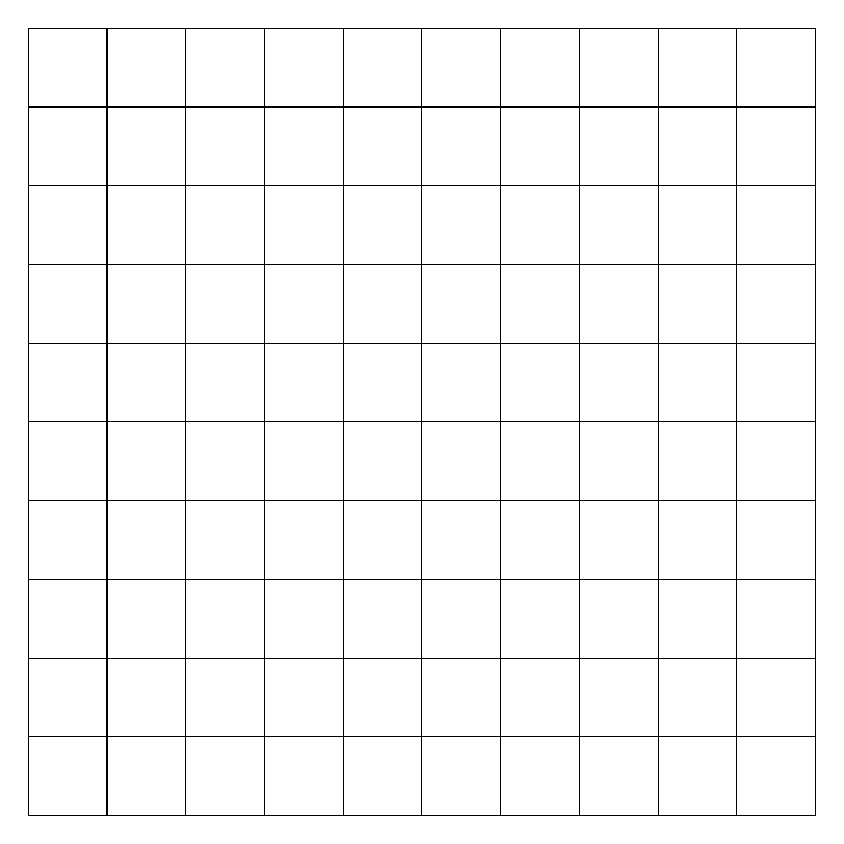
\begin{tikzpicture}
    \draw[step=\step] (0, 0) grid (10, 10);
    \parseSgf{\sgfA}
  \end{tikzpicture}
  \\
  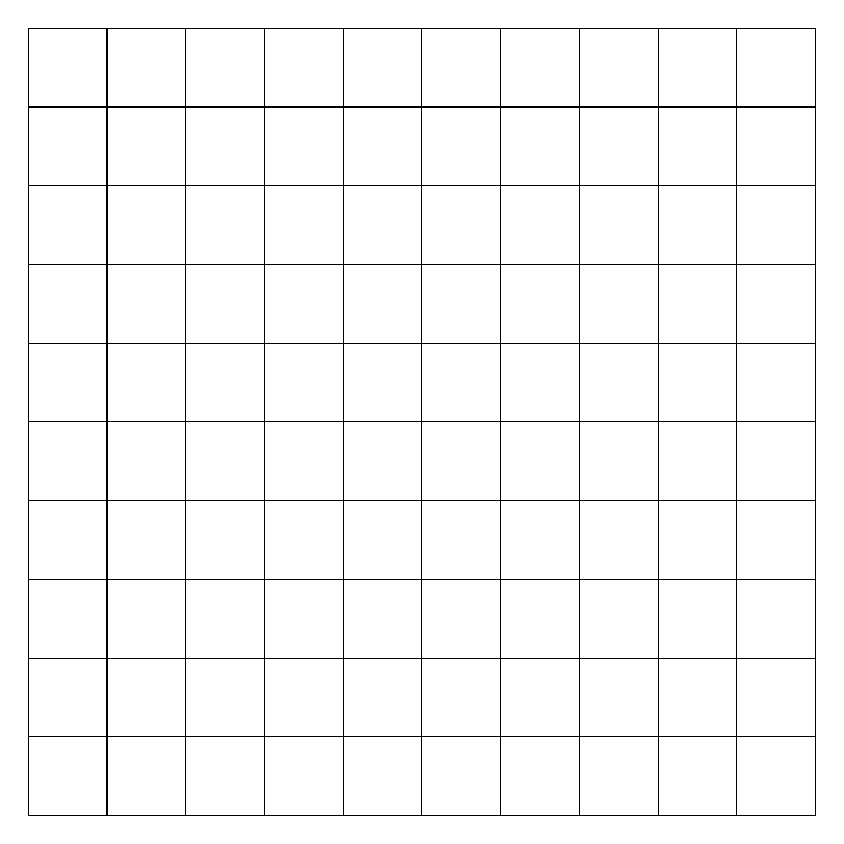
\begin{tikzpicture}
    \draw[step=\step] (0, 0) grid (10, 10);
    \parseSgf{\sgfB}
  \end{tikzpicture}
  \\
  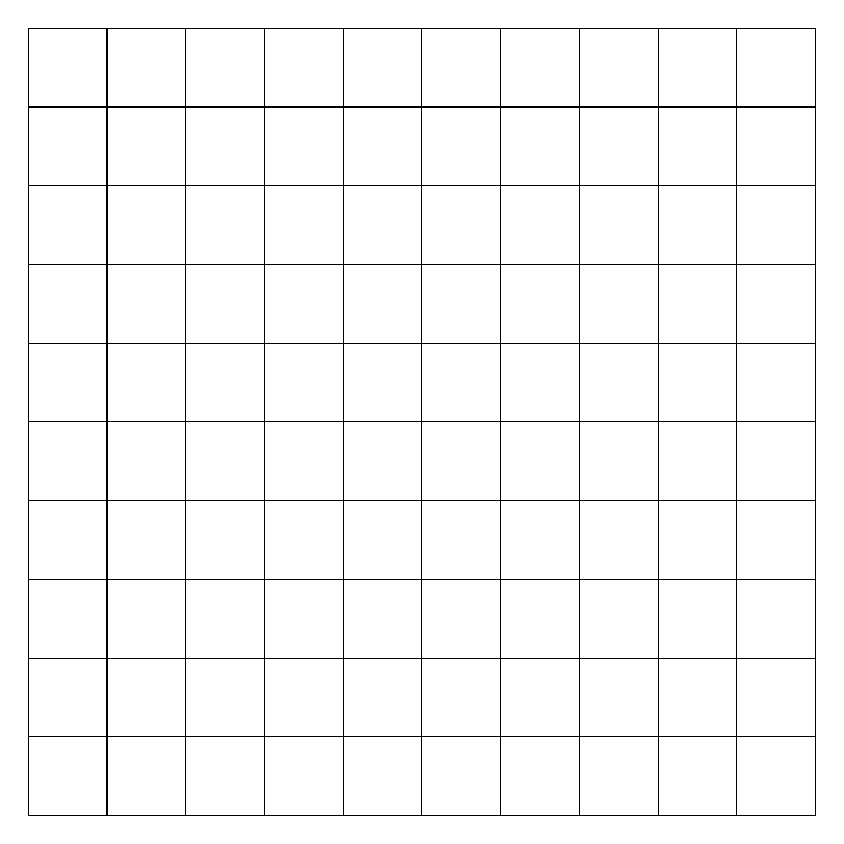
\begin{tikzpicture}
    \draw[step=\step] (0, 0) grid (10, 10);
    \parseSgf{\sgfA}
  \end{tikzpicture}
\end{document}